%%
%% Beuth Hochschule für Technik --  Abschlussarbeit
%%
%% Anhang
%%
%%%%%%%%%%%%%%%%%%%%%%%%%%%%%%%%%%%%%%%%%%%%%%%%%%%%%%%%%%%%%%%%%%%%%


\chapter{}

\section{Projektüberblick}\label{A.überblick}

\begin{figure}[h]
  \begin{center}
    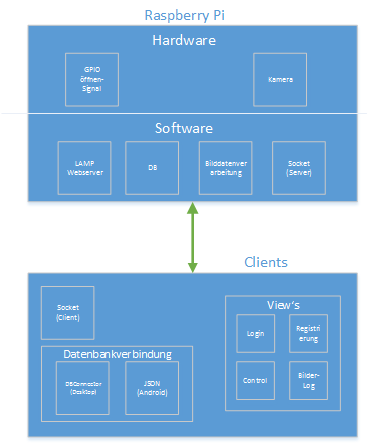
\includegraphics{ueberblick.png}
  		  %\caption{Wechseln zwischen Views}
     \label{fig.Views}
  \end{center}
\end{figure}



\newpage



\section{Desktopanwendung}\label{A.desktop}

\begin{figure}[h]
\begin{minipage}[h]{8cm}
	\centering
	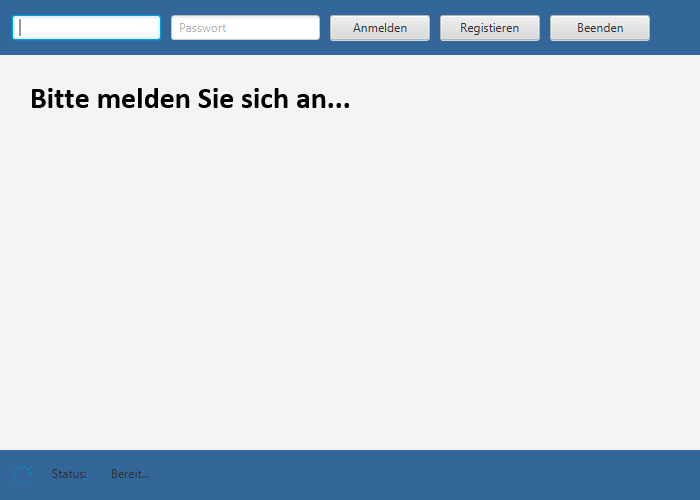
\includegraphics[width=\textwidth]{login.png}
	\caption{Login View}
\end{minipage}
\hfill
\begin{minipage}[h]{8cm}
	\centering
	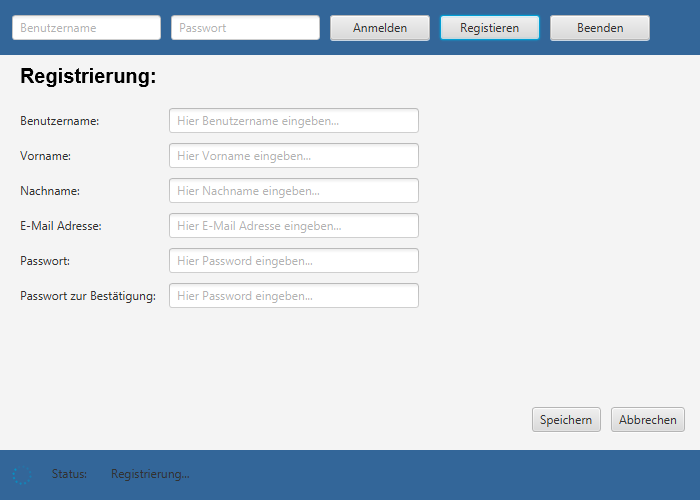
\includegraphics[width=\textwidth]{register.png}
	\caption{Datenbank View}
\end{minipage}
\end{figure}


\vspace{3cm}


\begin{figure}[h]
\begin{minipage}[h]{8cm}
	\centering
	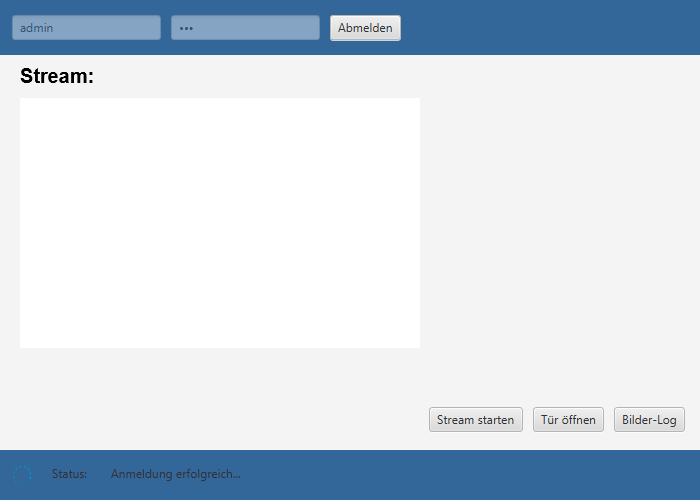
\includegraphics[width=\textwidth]{control.png}
	\caption{Control View ohne Stream}
\end{minipage}
\hfill
\begin{minipage}[h]{8cm}
	\centering
	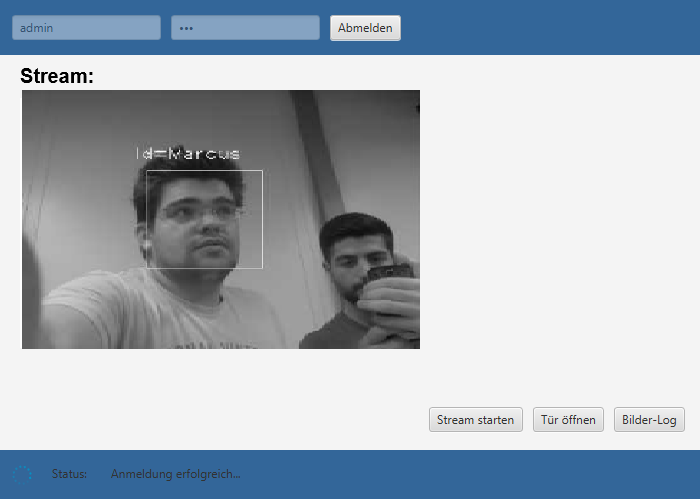
\includegraphics[width=\textwidth]{controlStream.png}
	\caption{Control View}
\end{minipage}
\end{figure}

\begin{figure}[ht]
  \begin{center}
    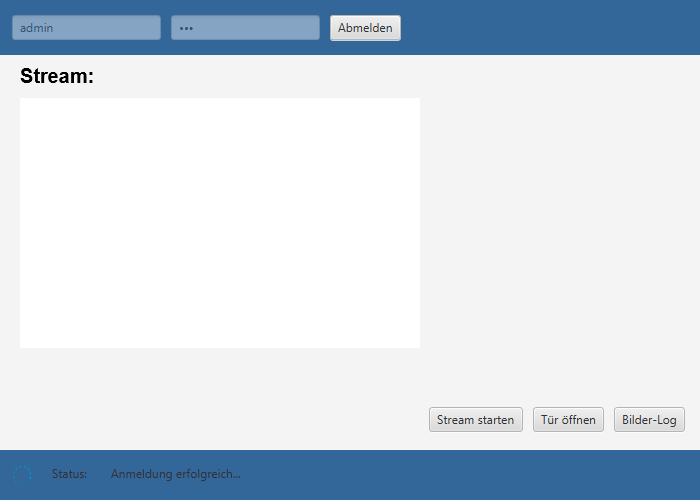
\includegraphics[scale=0.5]{control.png}
  		  \caption{Table View}
  \end{center}
\end{figure}


\newpage
\section{Android app}\label{A.android}


\begin{figure}[h]
\begin{minipage}[h]{8cm}
	\centering
	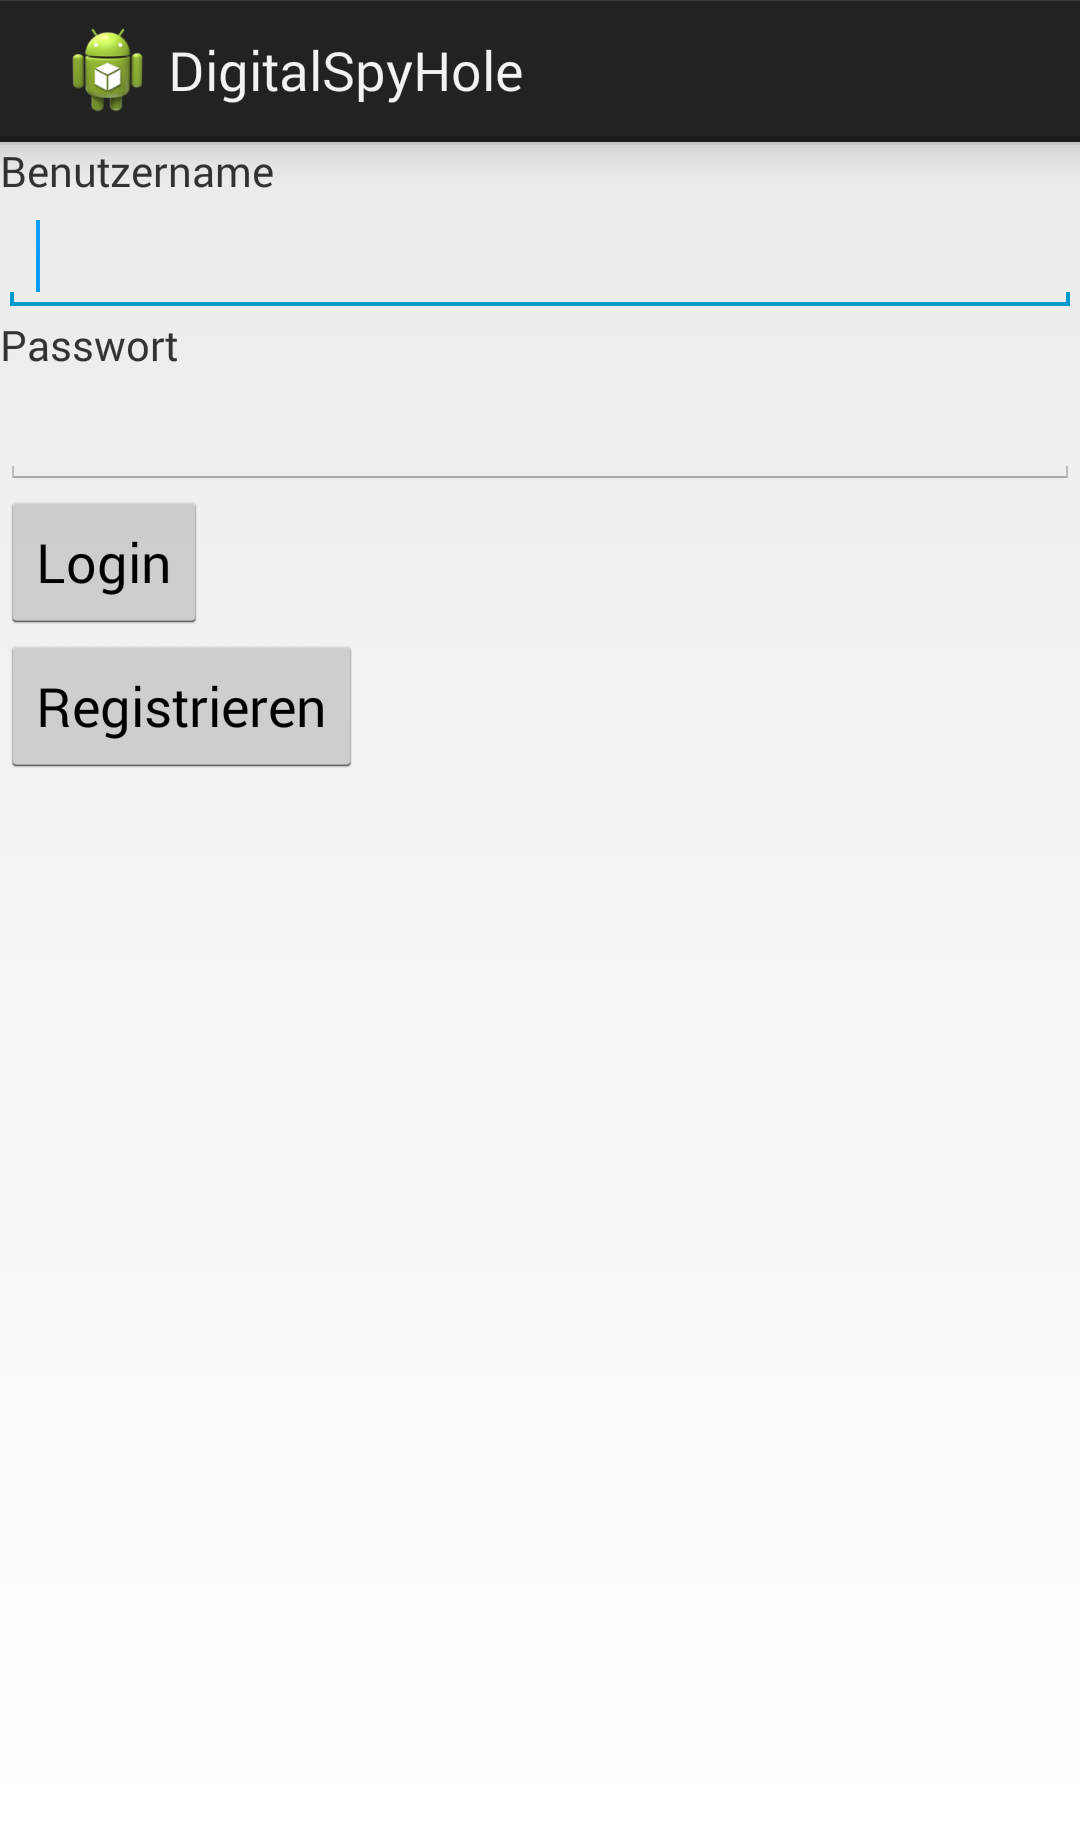
\includegraphics[scale=0.1]{2login.png}
	\caption{Login View}
\end{minipage}
\hfill
\begin{minipage}[h]{8cm}
	\centering
	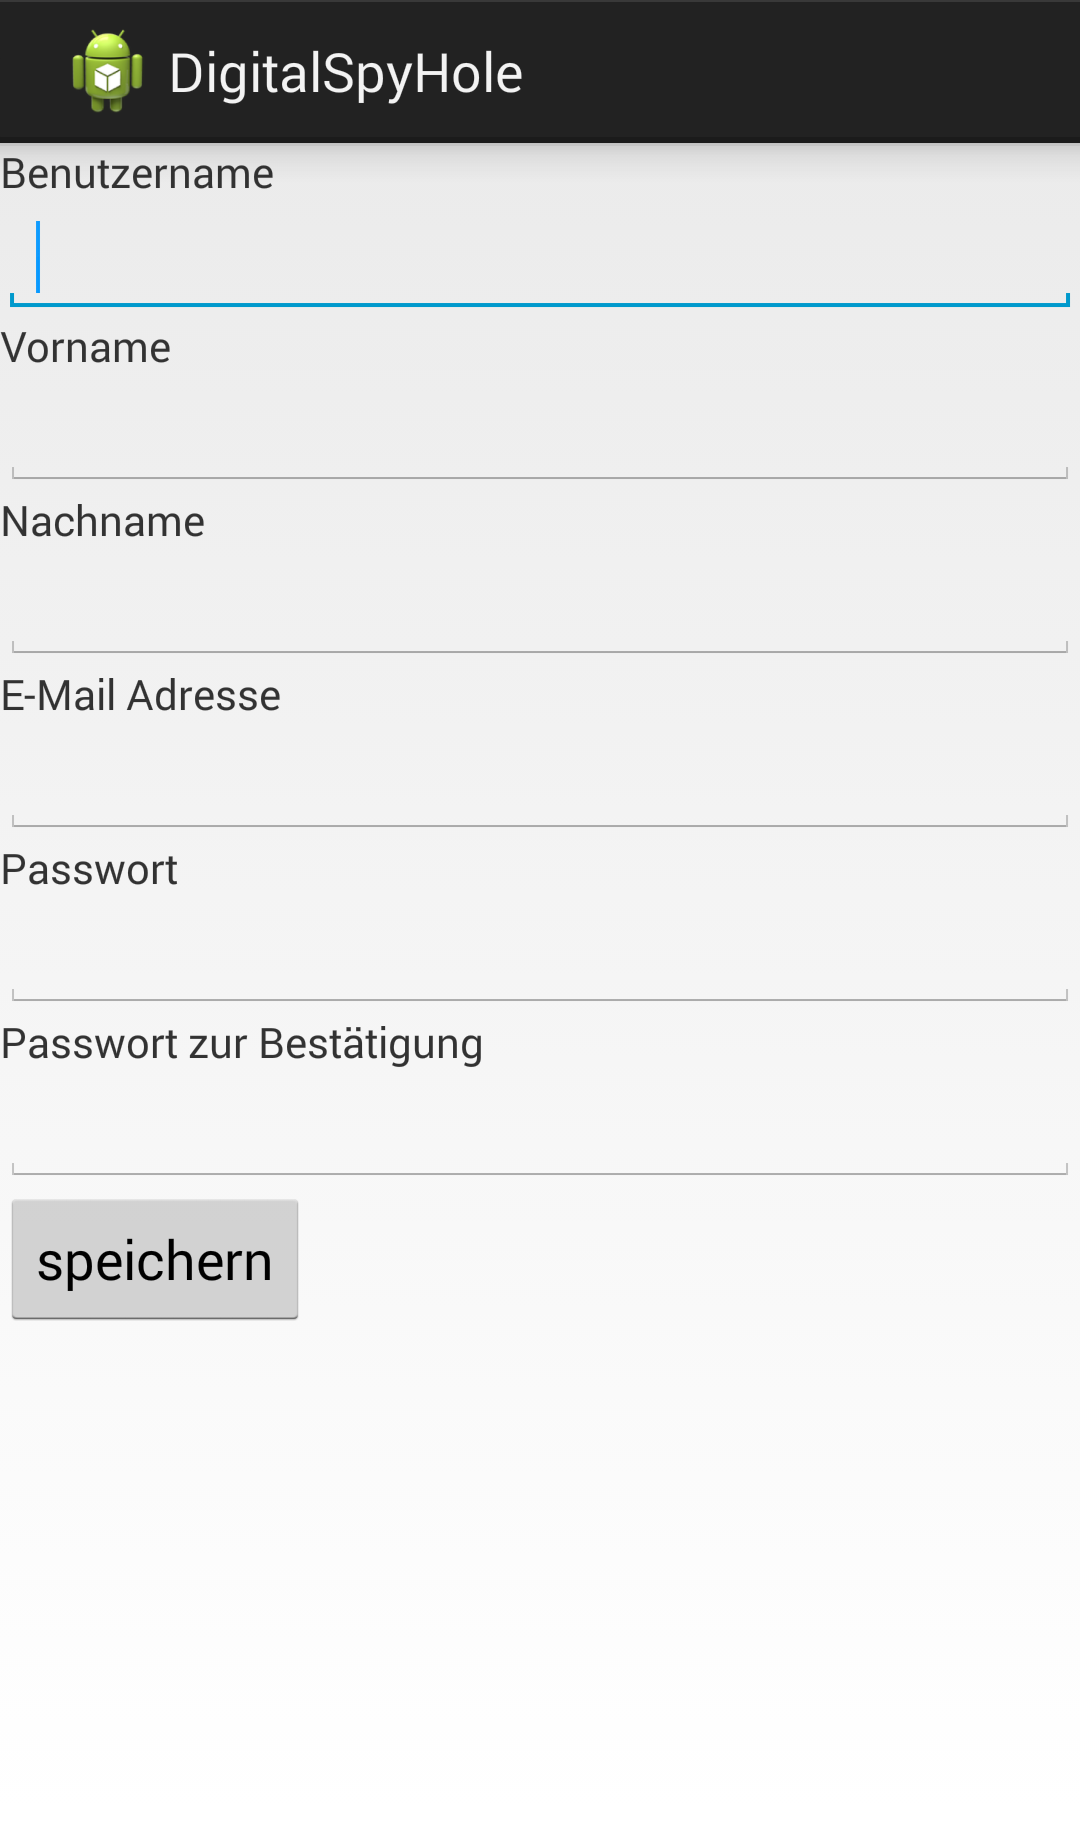
\includegraphics[scale=0.1]{21register.png}
	\caption{Registrierung View}
\end{minipage}
\end{figure}


\begin{figure}[h]
\begin{minipage}[h]{8cm}
	\centering
	%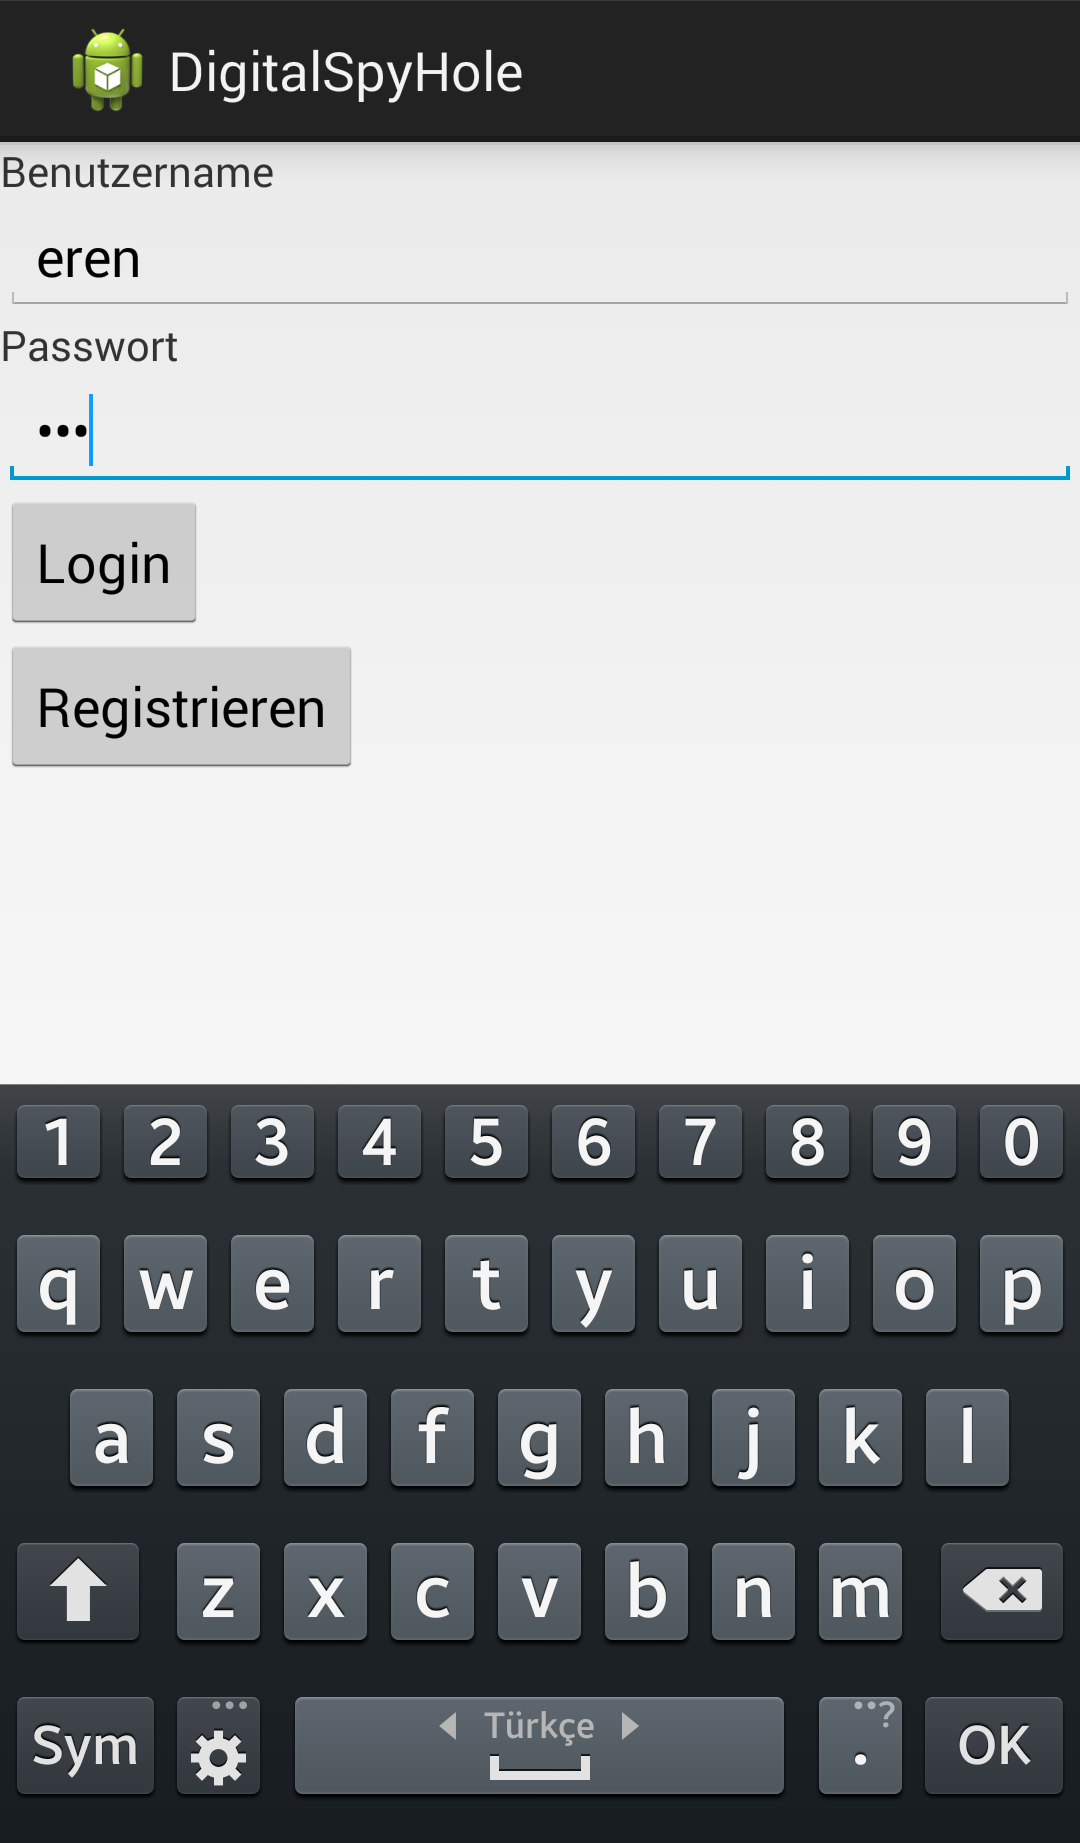
\includegraphics[width=\textwidth]{3logged.png}
	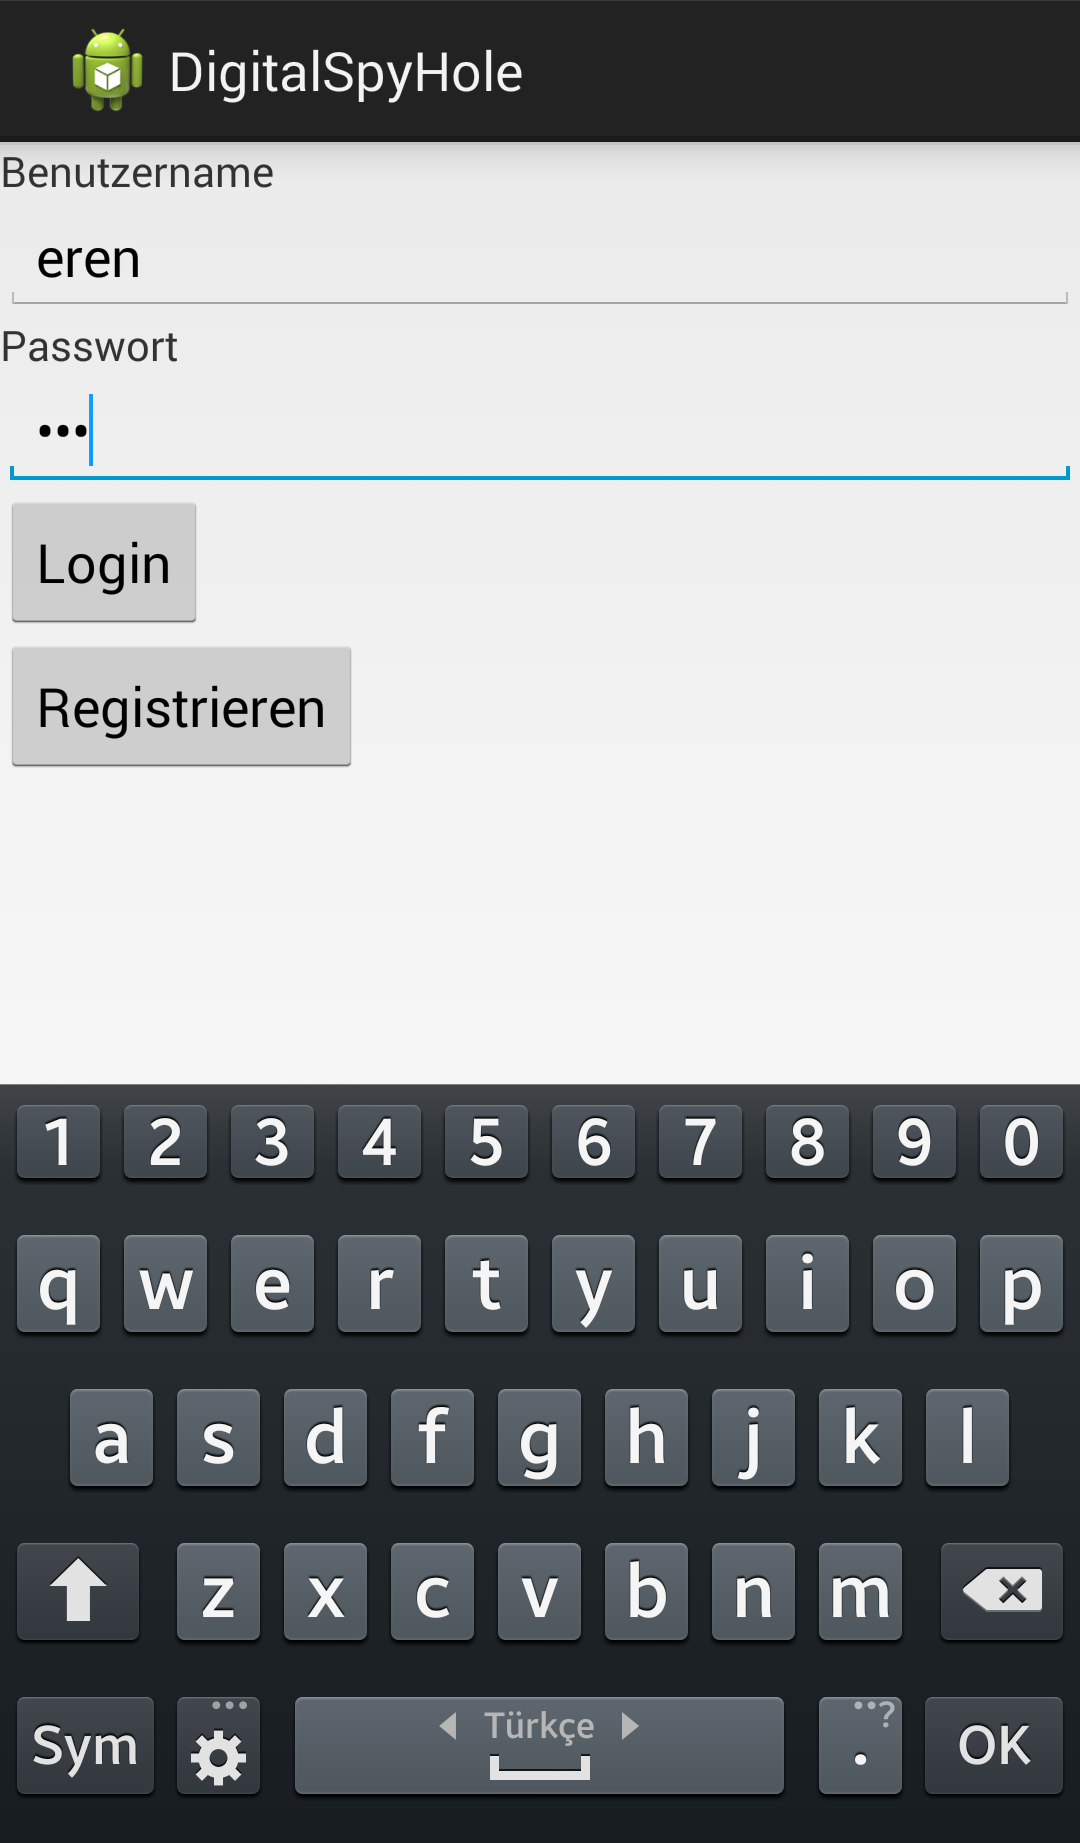
\includegraphics[scale=0.1]{3logged.png}
	\caption{Login View}
\end{minipage}
\hfill
\begin{minipage}[h]{8cm}
	\centering
	%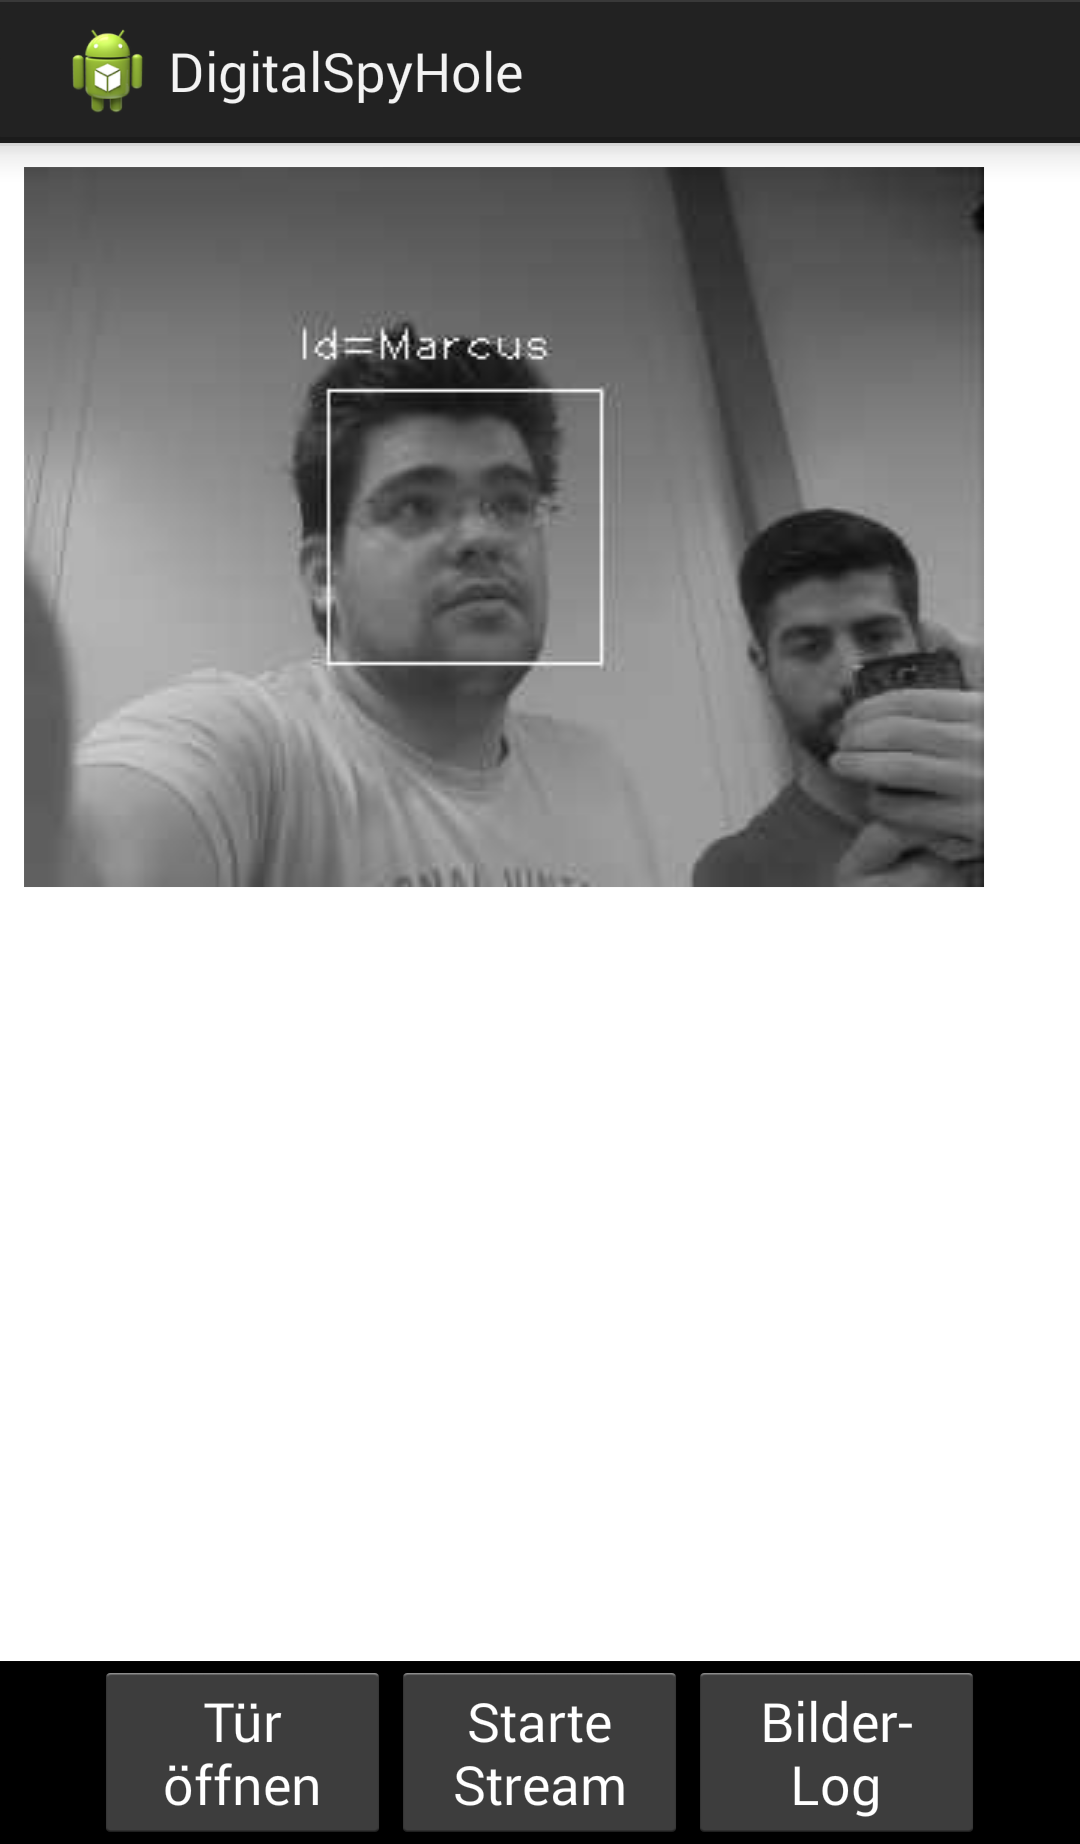
\includegraphics[width=\textwidth]{6stream.png}
	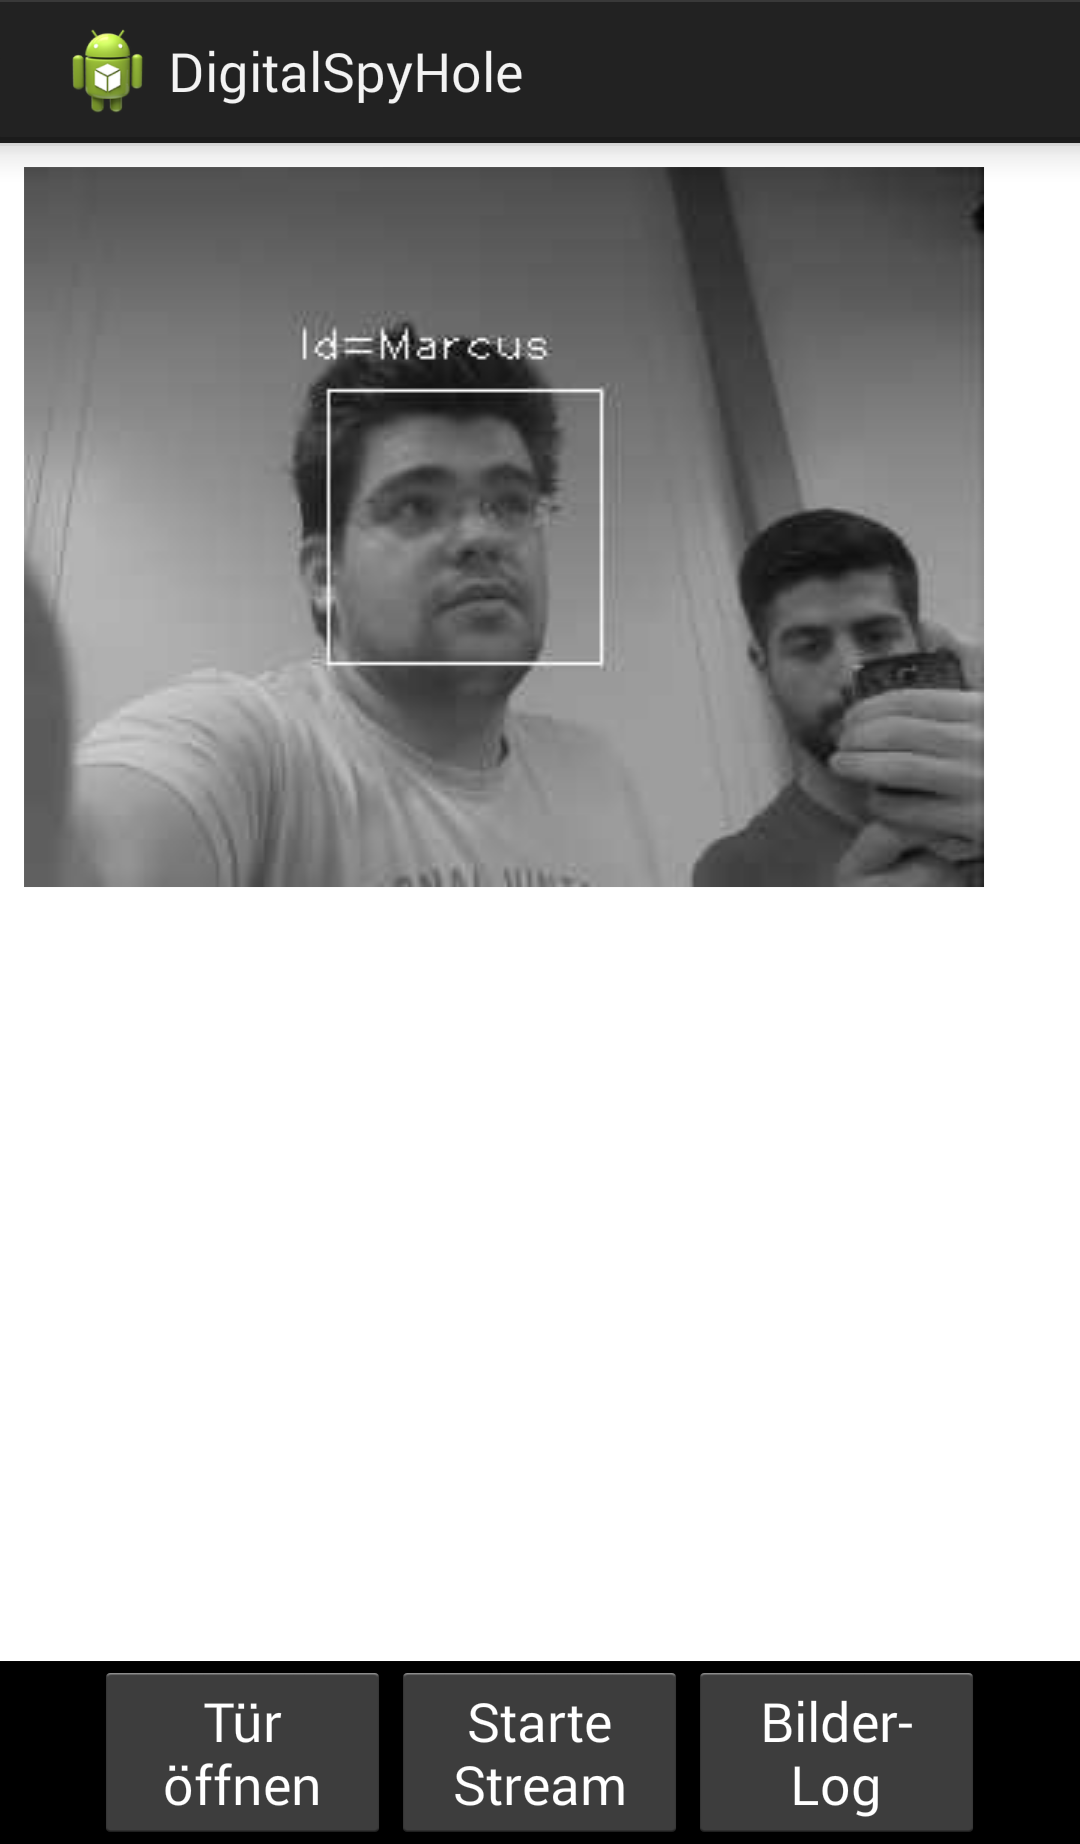
\includegraphics[scale=0.1]{6stream.png}
	\caption{Control View ohne Stream}
\end{minipage}
\end{figure}


\begin{figure}[ht]
  \begin{center}
    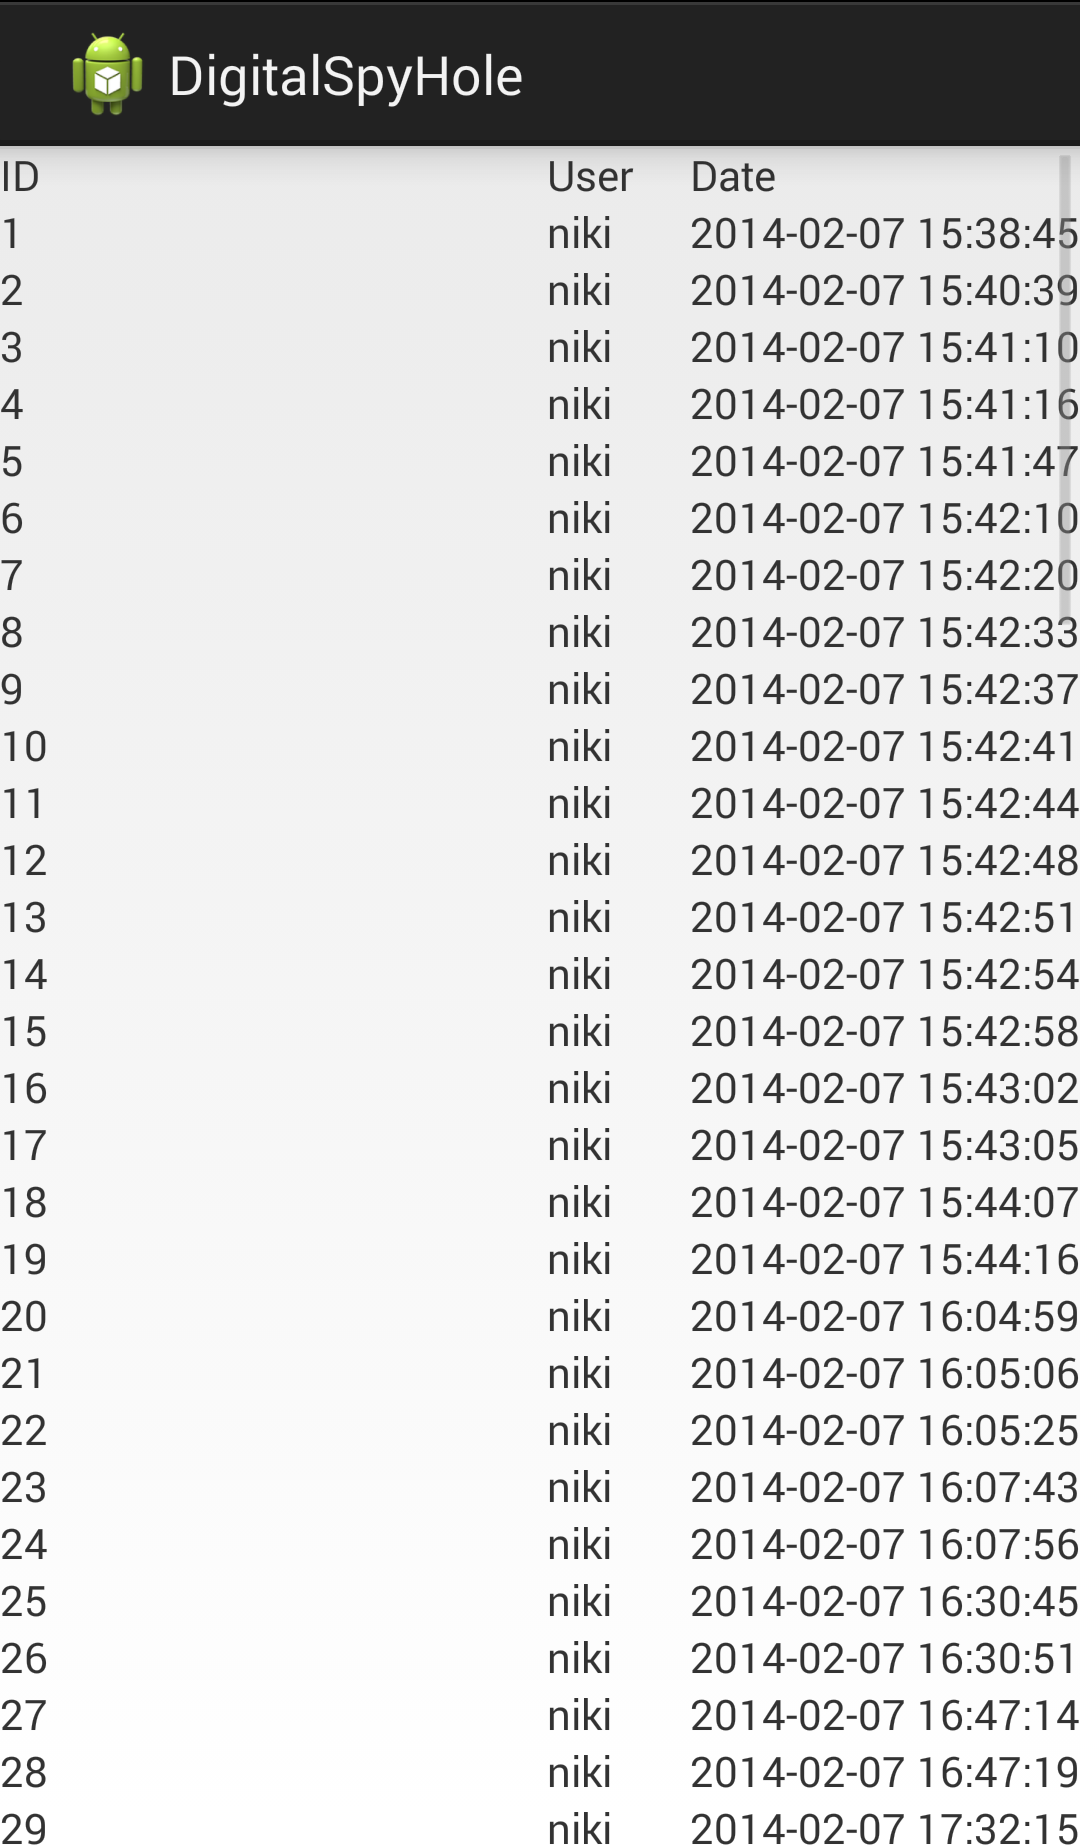
\includegraphics[scale=0.1]{5table.png}
  		  \caption{Table View}
  \end{center}
\end{figure}



